\documentclass[10pt,a4paper]{article}

\usepackage[margin=1.8cm]{geometry}
\usepackage{graphicx}
\usepackage{amsmath}
\usepackage{siunitx}
\usepackage{microtype}
\usepackage{caption}
\usepackage{parskip}
\usepackage{textcomp}
\usepackage{listings}
\usepackage[round]{natbib}   % author-year citations: \citet{} -> Author (year), \citep{} -> (Author, year)

\graphicspath{{results/}}   % figures in results/ (local); Overleaf also finds them next to this file
\setlength{\parindent}{0pt}
\captionsetup{font=small}
\sisetup{per-mode=power}   % units printed as µg m^-3

% Code appendix: upload rf_o3_cabauw_all.py next to this file (Overleaf).
% The literate line lets listings print the µ in the code.
\lstset{
  basicstyle=\ttfamily\scriptsize,
  breaklines=true,
  columns=fullflexible,
  frame=single,
  literate={µ}{{\textmu}}1
}

\begin{document}

\begin{center}
    {\Large \textbf{Meteorological Prediction of Hourly Ozone at Cabauw Using a Random Forest Model}}\\[0.3cm]
    \textbf{Thursina Muhammad Ahsan} \\
    Student number: 8256675
\end{center}

\section*{Introduction}

According to \citet{who2021}, surface ozone (O$_3$) is an important air pollutant that may damage lung function. It is formed through photochemical reactions involving precursor gases and solar radiation. This means, its concentration is strongly affected by meteorological condition \citep{otero2016}. O$_3$ typically has a daily cycle following the exposure to the solar radiation, it increases during daytime and lowers at night. This study investigates to predict the daily cycle of O$_3$ and to know to what extent meteorological variables alone can explain hourly O$_3$ cycle at Cabauw-Wielsekade station in the Netherlands using a random forest model.

\section*{Data and methods}

Hourly O$_3$ observations and meteorological data from Cabauw (NL10644) were used for 2016--2019. Cabauw location in a rural area is preferable to minimize local pollutant influences. Eight meteorological predictors were used: wind direction, wind speed, temperature, global radiation, hourly precipitation, pressure, cloud cover, and relative humidity.

% TODO (step 5): the assignment asks you to discuss WHY you chose this treatment of missing and negative values.
The dataset is pre-processed to remove hours containing missing O$_3$ or meteorological data, which amounts to 3.0\% of the data. The dataset also contains 608 negative O$_3$ measurements which were set to zero. The random forest model is configured with 30 trees and a minimum leaf size of five. It was trained on 25,450 hourly observations from 2016--2018 and then evaluated using 8,565 observations from 2019. The model performance was evaluated using correlation ($r$), $R^2$, root-mean-square error (RMSE), and mean bias. Additional experiments with varying number of trees (n = 10, 30, 100, 300) was done and also using each meteorological variable individually.
% TODO (consistency): "n" is also the cloud-cover variable in the data; consider another symbol or words.
% TODO (consistency): define the sign of the bias (predicted minus observed), so readers know negative = underestimate.
% TODO (step 15): AI acknowledgement for the code is required in the abstract.

\section*{Results and discussion}

\begin{figure}[h!]
    \centering
    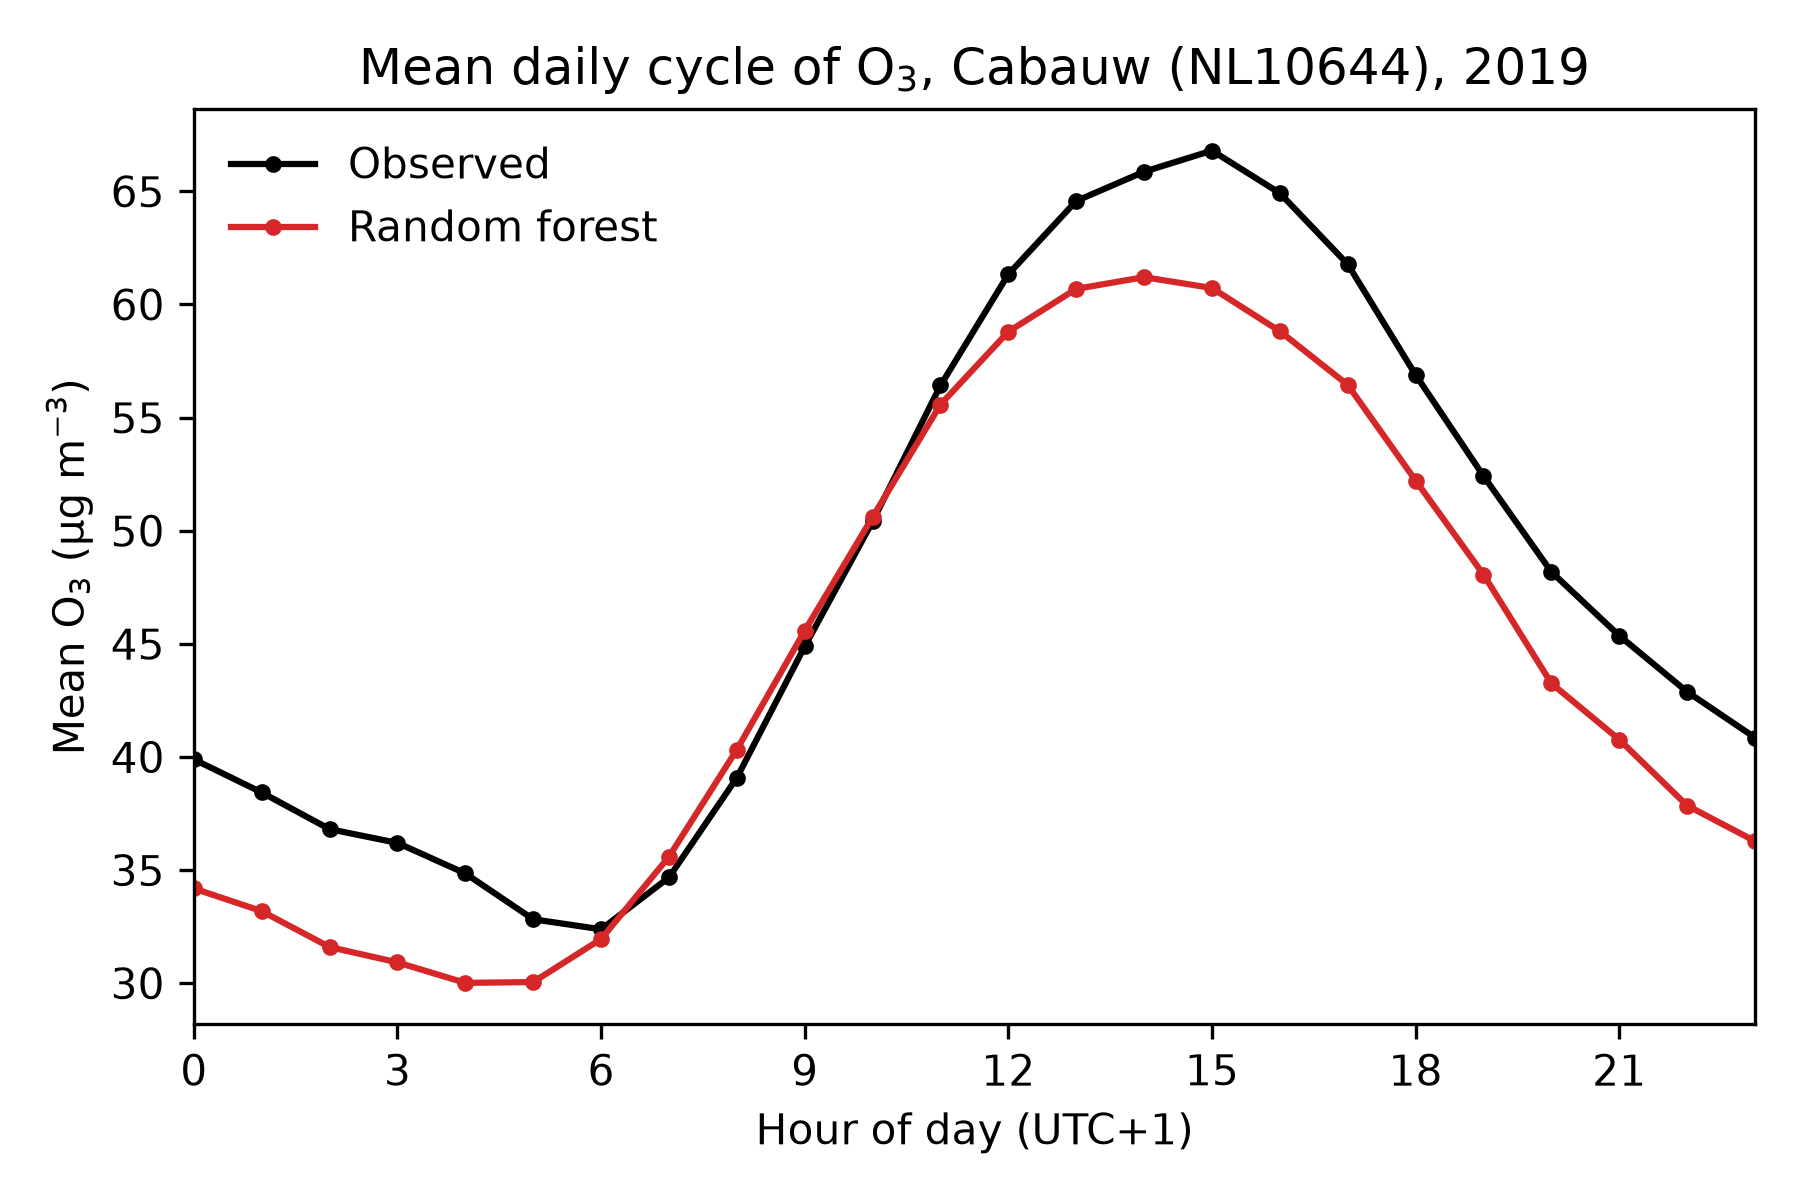
\includegraphics[width=0.50\textwidth]{fig_daily_cycle_2019.png}
    \caption{Mean daily cycle of O$_3$ at Cabauw during 2019. Black line shows observations and red line shows random-forest predictions.}
    \label{fig:daily}
\end{figure}

The model reproduced the training data well, with
$r=0.96$, $R^2=0.91$, and an RMSE of
\SI{8.1}{\micro\gram\per\cubic\metre}.
Then it evaluated to predict 2019 data, which produced
$r=0.87$, $R^2=0.74$, and an RMSE of
\SI{15.5}{\micro\gram\per\cubic\metre}.
% TODO (consistency): 47.9 - 44.5 = 3.4, but the bias is given as -3.5 (unrounded: 47.93 - 44.45 = 3.48).
Mean observed O$_3$ in 2019 was
\SI{47.9}{\micro\gram\per\cubic\metre},
compared with
\SI{44.5}{\micro\gram\per\cubic\metre}
predicted by the model, so there is a slight bias of
\SI{-3.5}{\micro\gram\per\cubic\metre} ($-7.3\%$).
The statistics difference between training and prediction performance indicates that  the model showed a decrease in predictive skill when applied outside the training period.

% TODO (consistency): model is below observations at 11-06 h (incl. the whole evening, 19-23 h)
% and slightly above at 07-10 h; check whether "night and late afternoon" describes this.
The model reproduced the overall daily O$_3$ cycle well (Fig.~\ref{fig:daily}), although the amplitude was slightly underestimated. The daytime increase is consistent with stronger photochemical production under higher radiation and temperature, together with changes in boundary-layer mixing. The model also tended to underestimate O$_3$ during the night and late afternoon.

The scatter plot shows that between hourly observations and predictions (Fig.~\ref{fig:scatter}), the model captures most of the variability, but it struggles to predict the higher concentrations \citep{fan2022}. The highest observed O$_3$ concentration in 2019 was \SI{258}{\micro\gram\per\cubic\metre}, whereas the maximum prediction was only
\SI{168}{\micro\gram\per\cubic\metre}.

\begin{figure}[h!]
    \centering
    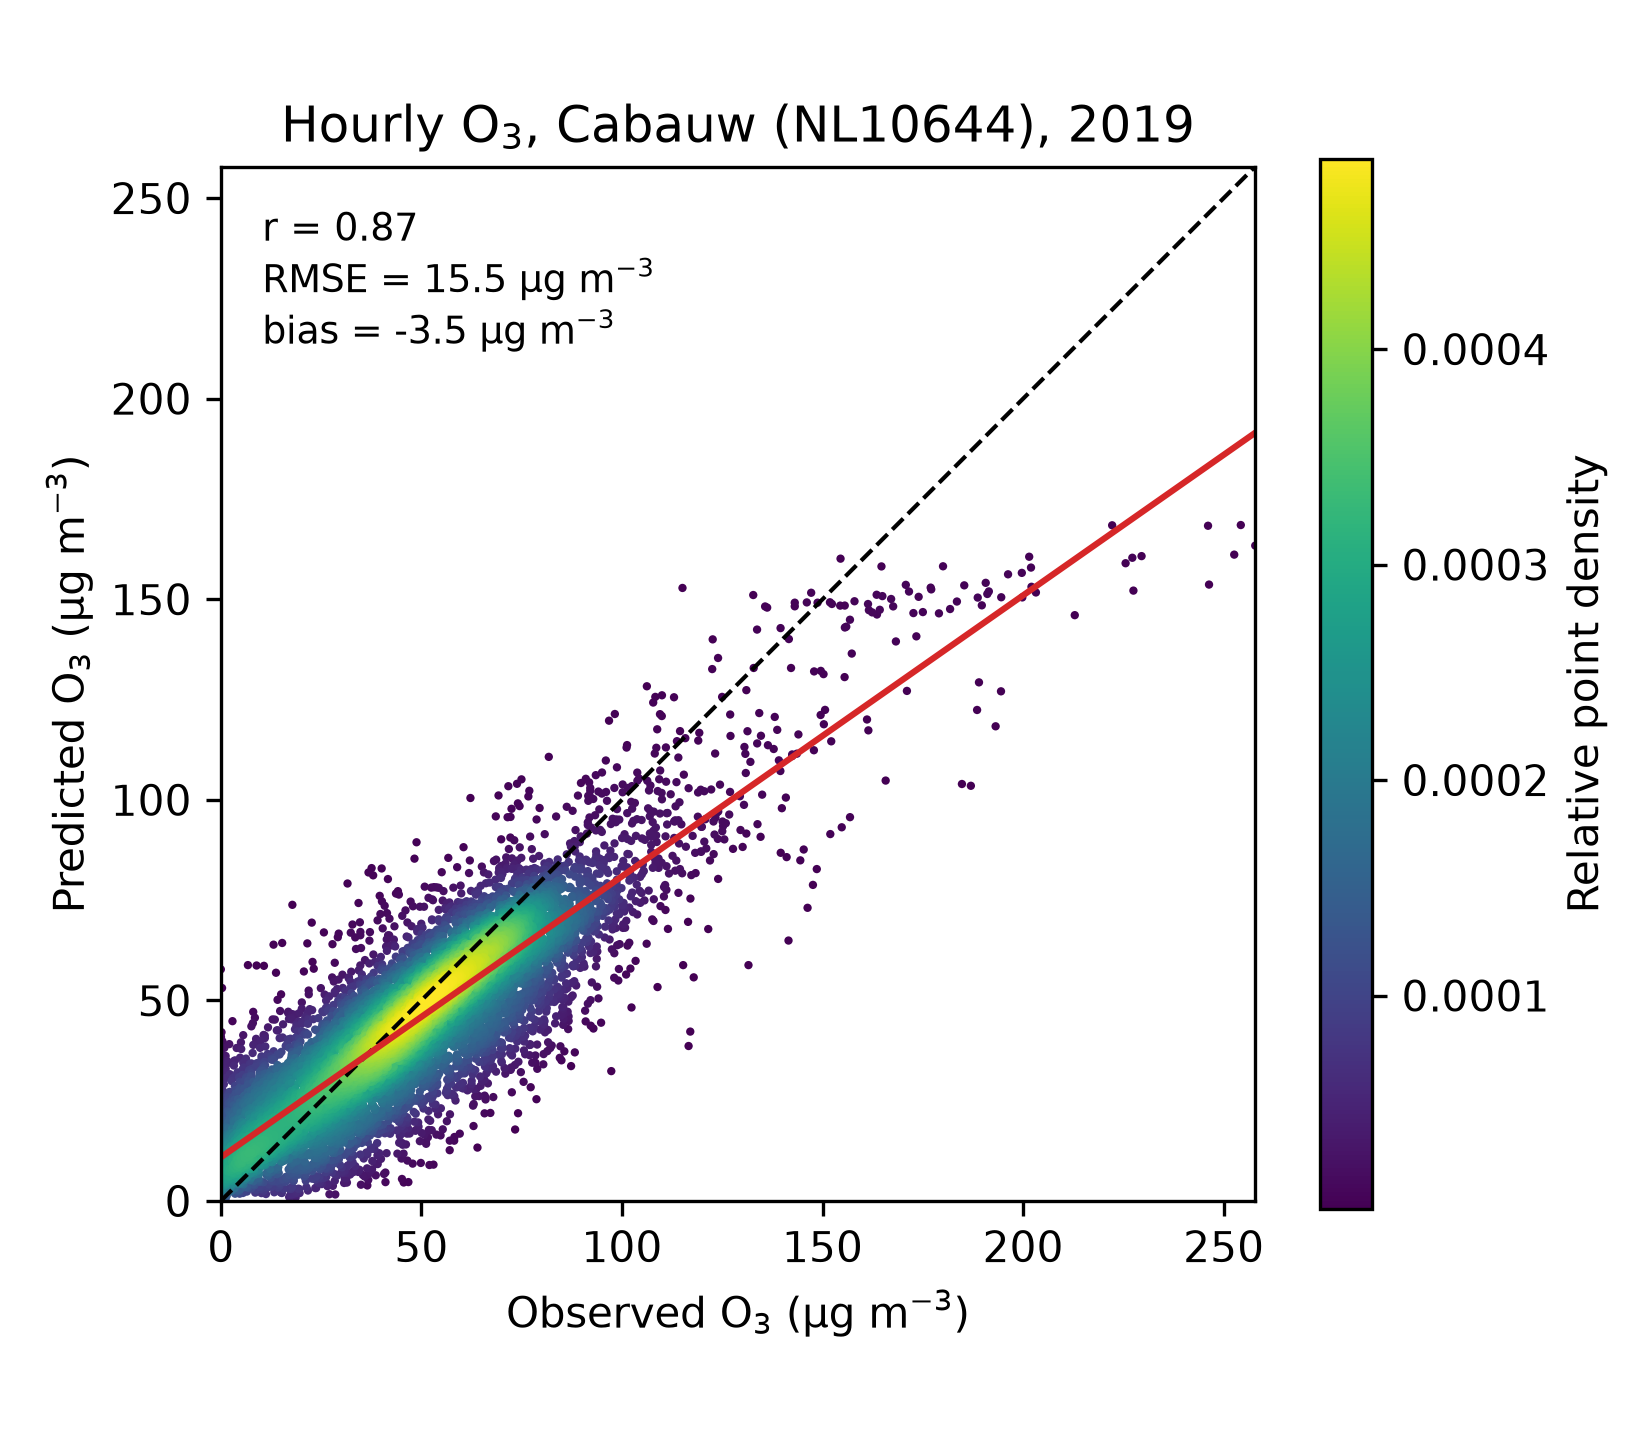
\includegraphics[width=0.65\textwidth]{fig_scatter_2019.png}
    \caption{Hourly predicted versus observed O$_3$ at Cabauw in 2019. Colour indicates point density, the dashed line represents 1:1 agreement, and the red line is the least-squares regression.}
    \label{fig:scatter}
\end{figure}

Increasing the number of trees had only a small effect on model performance. The RMSE decreased from \SI{15.80}{\micro\gram\per\cubic\metre} with 10 trees to \SI{15.54}{\micro\gram\per\cubic\metre} with 30 trees and \SI{15.42}{\micro\gram\per\cubic\metre} with 100--300 trees, while the correlation remained approximately constant at $r=0.87$.

% TODO (step 10): the assignment asks for the effects in terms of meteorology and chemistry (WHY rh, t, q).
% TODO (consistency): "significantly" suggests a statistical test, which was not done.
The single-variable experiments show that relative humidity was the strongest individual predictor, with $R^2=0.47$, $r=0.70$, and an RMSE of \SI{22.1}{\micro\gram\per\cubic\metre}, followed by temperature ($R^2=0.42$, $r=0.67$) and global radiation ($R^2=0.23$, $r=0.50$). The other meteorological parameters don't significantly explained the variability. In total, using all eight meteorological variables the model achieved $R^2=0.74$, which shows that there is no single meteorological variable that dominates the observed O$_3$ variability and there are other factors that influenced the concentration of O$_3$.

\section*{Conclusion}

% TODO (consistency): r = 0.87 and R^2 = 0.74 are statistics of all hourly 2019 values,
% not of the daily cycle (Fig. 1). Check that the sentence does not suggest they measure the daily-cycle fit.
This experiment shows that meteorology explains a substantial part of the hourly O$_3$ variability at Cabauw. For the 2019 data, the random forest model predicts daily cycle reasonably well, achieved $r=0.87$ and $R^2=0.74$. But it underestimated the mean concentration and the highest O$_3$ values. Relative humidity and temperature were the strongest individual predictors. Increasing the number of trees beyond n = 30 only showed minor improvements. Overall, the model captures the main meteorological control on O$_3$, but performs less well during extreme concentrations.

% Author-year labels: \bibitem[Short name(year)]{key}. Entries sorted alphabetically.
\begin{thebibliography}{3}

\bibitem[Fan et al.(2022)]{fan2022}
Fan, K., Dhammapala, R., Harrington, K., Lamastro, R., Lamb, B., and Lee, Y. (2022).
Development of a machine learning approach for local-scale ozone forecasting:
Application to Kennewick, WA.
\textit{Frontiers in Big Data}, 5, 781309.

\bibitem[Otero et al.(2016)]{otero2016}
Otero, N., Sillmann, J., Schnell, J. L., Rust, H. W., and Butler, T. (2016).
Synoptic and meteorological drivers of extreme ozone concentrations over Europe.
\textit{Environmental Research Letters}, 11, 024005.

\bibitem[WHO(2021)]{who2021}
World Health Organization (2021).
\textit{WHO global air quality guidelines: particulate matter (PM$_{2.5}$ and PM$_{10}$), ozone, nitrogen dioxide, sulfur dioxide and carbon monoxide.}
Geneva: World Health Organization.

\end{thebibliography}
\label{abstractend}   % marks the last page of the abstract (before the appendix)

\clearpage
\section*{Appendix: Python code}
\lstinputlisting[language=Python]{rf_o3_cabauw_all.py}

\end{document}
